%%%%%%%%%%%%%%%%%%%%%%%%%%%%%%%%%%%%%%%%%%%%%%%%%%%%%%%%%%%%%%%%
%%%%%%%%%%%%%%%%%%%%%%%%%%%%%%%%%%%%%%%%%%%%%%%%%%%%%%%%%%%%%%%%
%%%%
%%%% This text file is part of the source of 
%%%% `Introduction to High-Performance Scientific Computing'
%%%% by Victor Eijkhout, copyright 2012-8
%%%%
%%%% This book is distributed under a Creative Commons Attribution 3.0
%%%% Unported (CC BY 3.0) license and made possible by funding from
%%%% The Saylor Foundation \url{http://www.saylor.org}.
%%%%
%%%%
%%%%%%%%%%%%%%%%%%%%%%%%%%%%%%%%%%%%%%%%%%%%%%%%%%%%%%%%%%%%%%%%
%%%%%%%%%%%%%%%%%%%%%%%%%%%%%%%%%%%%%%%%%%%%%%%%%%%%%%%%%%%%%%%%

In section~\ref{sec:block-algebra} you saw that certain linear algebra
algorithms can be formulated in terms of submatrices. This point of
view can be beneficial for the efficient execution of linear algebra
operations on shared memory architectures such as current
\indexterm{multicore} processors.

\newcommand\chol{\mathop{\mathrm{Chol}}}
As an example, let us consider the \indexterm{Cholesky factorization},
which computes $A=LL^t$ for a symmetric positive definite matrix~$A$;
see also section~\ref{sec:cholesky}.
Recursively, we can describe the algorithm as follows:
\[ \chol
\begin{pmatrix}
  A_{11}&A_{21}^t\\ A_{21}&A_{22}
\end{pmatrix} = LL^t\qquad\hbox{where}\quad L=
\begin{pmatrix}
  L_{11}&0\\ \tilde A_{21} &\chol(A_{22}-\tilde A_{21}\tilde A_{21}^t)
\end{pmatrix}
\]
and where $\tilde A_{21}=A_{21}L_{11}\invt,$ $A_{11}=L_{11}L_{11}^t$.

In practice, the block implementation is applied to a partitioning
\[
\left(
\begin{array}{c|c|cc}
  &\multicolumn{2}{c}{\mathrm{finished}}\\ \hline
  \multirow{2}{*}{}&A_{kk}&A_{k,>k}&\\ \hline
  &A_{>k,k}&A_{>k,>k}
\end{array}
\right)
\]
where $k$ is the index of the current block row, and the
factorization is finished for all indices~$<k$.
The factorization is written as follows,
using Blas names for the operations:
\begin{quotation}
  \begin{tabbing}
    for \=$k=1,\mathrm{nblocks}$:\\
    \>\n{Chol}: factor $L_kL_k^t\leftarrow A_{kk}$\\
    \>\n{Trsm}: solve $\tilde A_{>k,k} \leftarrow A_{>k,k}L_k\invt$\\
    \>\n{Gemm}: form the product $\tilde A_{>k,k}\tilde A_{>k,k}^t$\\
    \>\n{Syrk}: symmmetric rank-$k$ update
    $A_{>k,>k}\leftarrow A_{>k,>k}-\tilde A_{>k,k}\tilde A_{>k,k}^t$
  \end{tabbing}
\end{quotation}
The key to parallel performance is to partition the indices~$>k$ and
write the algorithm in terms of these blocks:
\[
\left(
\begin{array}{c|c|cc}
  &\multicolumn{2}{c}{\mathrm{finished}}\\ \hline
  \multirow{2}{*}{}&A_{kk}&A_{k,k+1}&A_{k,k+2}\cdots\\ \hline
  &A_{k+1,k}&A_{k+1,k+1}&A_{k+1,k+2}\cdots\\
  &A_{k+2,k}&A_{k+2,k+2}\\
  &\vdots&\vdots
\end{array}
\right)
\]
The algorithm now gets an extra level of inner loops:
\begin{quotation}
  \begin{tabbing}
    for \=$k=1,\mathrm{nblocks}$:\\
    \>\n{Chol}: factor $L_kL_k^t \leftarrow A_{kk}$\\
    \>for \=$\ell>k$:\\
    \>\>\n{Trsm}: solve $\tilde A_{\ell,k} \leftarrow A_{\ell,k}L_k\invt$\\
    \>for \=$\ell_1,\ell_2>k$:\\
    \>\>\n{Gemm}: form the product $\tilde A_{\ell_1,k}\tilde A_{\ell_2,k}^t$\\
    \>for \=$\ell_1,\ell_2>k$, $\ell_1\leq\ell_2$:\\
    \>\>\n{Syrk}: symmmetric rank-$k$ update
    $A_{\ell_1,\ell_2}\leftarrow A_{\ell_1,\ell_2}
    -\tilde A_{\ell_1,k}\tilde A_{\ell_2,k}^t$
  \end{tabbing}
\end{quotation}

\begin{figure}[ht]
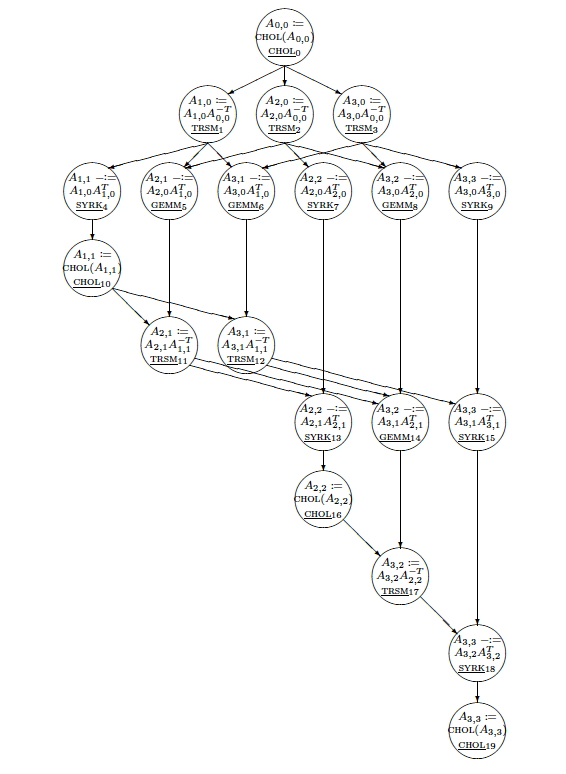
\includegraphics[scale=.7]{graphics/chol4dag}
  \caption{Graph of task dependencies in a $4\times4$ Cholesky
    factorization}
  \label{fig:chol4dag}
\end{figure}

Now it is clear that the algorithm has a good deal of parallelism: the
iterations in every $\ell$-loop can be processed independently.
However, these loops get shorter in every iteration of the outer
$k$-loop, so it is not immediate how many processors we can
accommodate. Moreover, it is not necessary to preserve the order of
operations of the algorithm above. For instance, after
\[
  L_1L_1^t=A_{11},\quad A_{21}\leftarrow A_{21}L_1\invt,\quad
  A_{22}\leftarrow A_{22}-A_{21}A_{21}^t
\]
the factorization $L_2L_2^t=A_{22}$ can start, even if the rest of the
$k=1$ iteration is still unfinished. Thus, there is probably a lot more
parallelism than we would get from just parallelizing the inner loops.

The best way to approach parallelism in this case is to shift away
from a \indexterm{control flow} view of the algorithm, where the
sequence of operations is prescribed, to a \indexterm{data flow} view.
In the latter only data dependencies are indicated, and any ordering of
operations that obeys these dependencies is allowed. (Technically, we
abandon the program order of the tasks and replace it with a
\indexterm{partial ordering}
\begin{footnoteenv}
{Let's write $a\leq b$ if $a$~is
  executed before~$b$, then the relation~$\cdot\leq\cdot$ is a partial
  order if $a\leq b\wedge b\leq a\Rightarrow a=b$ and $a\leq b\wedge
  b\leq c\Rightarrow a\leq c$. The difference with a total ordering,
  such as program ordering, is that it is not true that $a\leq b\vee
  b\leq a$: there can be pairs that are not ordered, meaning that
  their time ordering is not prescribed.}
  \end{footnoteenv}
  .)  The best way of
representing the data flow of an algorithm is by constructing a
\indexacf{DAG} (see section~\ref{app:graph} for a brief tutorial on
graphs) of tasks.  We add an edge $(i,j)$ to the graph if task~$j$
uses the output of task~$i$.

\begin{exercise}
  In section~\ref{sec:seq-consist} you learned the concept of
  \indexterm{sequential consistency}: a threaded parallel code program
  should give the same results when executed in parallel as when it's
  executed sequentially. We have just stated that \ac{DAG}-based
  algorithms are free to execute tasks in any order that obeys the
  partial order of the graph nodes. Discuss whether
  sequential consistency is a problem in this context.
\end{exercise}

In our example, we construct a \ac{DAG} by making a vertex task for every
inner iteration.
Figure~\ref{fig:chol4dag} shows the \ac{DAG} of all tasks
of matrix of $4\times4$ blocks. This graph is constructed by
simulating the Cholesky algorithm above, 

\begin{exercise}
  What is the diameter of this graph? Identify the tasks that lie on
  the path that determines the diameter. What is the meaning of these
  tasks in the context of the algorithm? This path is called the
  \indexterm{critical path}. Its length determines the execution time of the
  computation in parallel, even if an infinite number of processors is
  available.
\end{exercise}

\begin{exercise}
  Assume there are $T$ tasks that all take a unit time to execute, and
  assume we have $p$ processors. What is the
  theoretical minimum time to execute the algorithm? Now amend this
  formula to take into account the critical path; call its length~$C$.
\end{exercise}

In the execution of the tasks a \ac{DAG}, several observations
can be made.
\begin{itemize}
\item If more than one update is made to a block, it is probably
  advantageous to have these updates be computed by the same
  process. This simplifies maintaining \indextermbus{cache}{coherence}.
\item If data is used and later modified, the use must be finished
  before the modification can start. This can even be true if the two
  actions are on different processors, since the memory subsystem
  typically maintains cache coherence, so the modifications can affect the
  process that is reading the data. This case can be remedied by
  having a copy of the data in main memory, giving a reading process
  data that is reserved (see section~\ref{sec:coherence}).
\end{itemize}

\endinput

The concept of lookahead has been to used to parallelize operations
such as the $LU$ factorization.
The $LU$ factorization subproblem performed within each iteration of
the loop updates a block on the diagonal of the matrix $A_{kk}$.
With the exception of the first iteration, this diagonal block is
previously updated by a 
matrix-matrix multiplication update.
For instance,
$A_{22} \leftarrow A_{22} - A_{21} A_{12}$ resides within the first
iteration while
$A_{22} \leftarrow LU( A_{22} )$ resides within the second iteration.
As we noted above, each of these updates can be paralleled in
parallel, so lookahead attempts to schedule the block update on the
diagonal first.
Once that block is updated, the $LU$ subproblem is ``computed ahead''
of its current iteration in parallel with the remaining block updates
from the current iteration.
This process can be done repeated for multiple iterations ahead of the
current iteration in order to exploit more opportunities for
parallelism.

The difficulty with adopting lookahead is that it introduces
unnecessary complexity into the code that implements the linear
algebra algorithms.
We focus on a different methodology that parallelizes matrix computations
using a separation of concerns.
Instead of executing operations on blocks immediately, the tasks are
stored by a runtime system.
As tasks are stored, data dependencies between each task are computed.
If we view tasks as nodes in a graph and data dependencies as the
edges, a \acf{DAG} is implicitly formed.
Once all the tasks are stored and the \ac{DAG} is fully constructed, the
runtime system then schedules and dispatches tasks to threads in
parallel.

$LU$ factorization without pivoting only exhibits read-after-write, or
flow, dependencies where one task will update a block and then a
subsequent task will read the value of that updated block.
For instance,
$A_{11} \leftarrow LU( A_{11} )$ overwrites the block $A_{11}$
while each multiplication 
$A_{i1} \leftarrow A_{i1} A_{11}^{-1}$ where $1 < i \leq M$
reads the updated block $A_{11}$. %(good notation?)
This situation leads to flow dependencies between the task
encapsulating the first $LU$ factorization subproblem and the
proceeding triangular solve tasks.
%(have we introduced trsm yet?).
The process for detecting data dependencies between tasks is automated
by the runtime system.

In figure~\ref{fig:dag} we present the \ac{DAG} for $LU$ factorization
without pivoting given a 
$3 \times 3$ matrix of blocks.
We can clearly see that many opportunities for parallelism exist with
the \ac{DAG}.
For example, the tasks 
$A_{21} \leftarrow A_{21} A_{11}^{-1}$,
$A_{31} \leftarrow A_{31} A_{11}^{-1}$,
$A_{12} \leftarrow A_{11}^{-1} A_{12}$, and
$A_{13} \leftarrow A_{11}^{-1} A_{13}$
can all be scheduled in parallel.

Many different scheduling algorithms and heuristics can be applied to
schedule and dispatch tasks.
A simple scheduling algorithm is to use a single first-in first-out
(FIFO) queue.
All tasks that are ready to execute are enqueued onto this single
queue.
Once a particular thread dequeues a task and executes it, all the
dependent tasks are notified, and any newly ready tasks are enqueued.
For instance,
The task $A_{11} \leftarrow LU( A_{11} )$ is executed by a thread and
then notifies its four dependent tasks
$A_{21} \leftarrow A_{21} A_{11}^{-1}$,
$A_{31} \leftarrow A_{31} A_{11}^{-1}$,
$A_{12} \leftarrow A_{11}^{-1} A_{12}$, and
$A_{13} \leftarrow A_{11}^{-1} A_{13}$,
all of which become ready and thus enqueued.
This process of scheduling and dispatching tasks is done until all
tasks have been executed.

This single FIFO queue scheduling provides a near optimal load balance
of threads since any idle thread will attempt to dequeue a task
whenever one is available.
Instead of using a FIFO ordering of the single queue, a priority queue
can be used where the tasks on the queue can be sorted according to
different heuristics.
One certain heuristic attempts to reduce the critical path of
execution by using the heights of each task within the \ac{DAG} where the
height of a task is defined as the distance of a node to its farthest
leaf.  %(Graph theory in appendix right?)
This heuristic mimics lookahead and is encapsulated within the runtime
system without introducing complexity into the $LU$ factorization
code.

Since each of the task operands are matrix blocks, data locality is
another key component to an efficient scheduling of tasks along with
load balance.
A single FIFO queue does not address data locality since any task can
execute on nearly any thread.
More sophisticated scheduling algorithms attempt to address load
balance and data locality simultaneously.

\begin{figure}
\begin{center}
DAG
\end{center}
\caption{The directed acyclic graph for $LU$ factorization without
  pivoting given a $3 \times 3$ matrix of blocks.}
\label{fig:dag}
\end{figure}
